\chapter{Discrete Mechanics For Rigid Bodies On Lie Groups}

\section{Discrete Lagrangian Mechanics}
\label{section:discrete_lagrangian_mechanics}

\subsection{Discrete Euler-Lagrange Equations}

\begin{proposition}[Directional derivative representation of $D_{g_k}L_d(g_k,f_k)$]
Let $G$ be a Lie group with Lie algebra $\mathfrak g$ \cite{Hall2000LieGroups}. Let 
$L_d:G\times G\to\mathbb R$ be smooth and $\eta_k$ an arbitrary element of $\mathfrak g$. For all $\delta g_k\in T_{g_k}G$ with $\delta g_k = T_eL_{g_k}(\eta_k)$ \eqref{eq:VARIATION},
we regard the partial derivative $D_{g_k}L_d(g_k,f_k)\in T_{g_k}^*G$ as the covector characterized by
\begin{equation} \label{eq:derivative_gk}
\langle D_{g_k}L_d(g_k,f_k),\delta g_k\rangle
=
\langle T_{e}^{*}L_{g_k} D_{g_k}L_d(g_k,f_k),\eta_k \rangle
=
\left.\frac{d}{d\varepsilon}\right|_{\varepsilon=0}L_d(g_k\exp{(\varepsilon \eta_k)},f_k).
\end{equation}
\end{proposition}

\begin{proof}
Since $G$ is a smooth manifold, the differential of the map $L_d(g_k,f_k)$ is a linear map
$T_{g_k}G\to\mathbb R$, as $f_k$ is fixed. Therefore, the partial derivative
$D_{g_k}L_d(g_k,f_k)$ is an element of the dual space $T_{g_k}^*G$. Moreover, for any
$\eta_k \in \mathfrak g$, let
\[
\gamma(\varepsilon)=g_k\exp{(\varepsilon \eta_k)}
\]
be a smooth curve on the manifold. Then
$\gamma(0)=g_k$ and
\begin{align} \label{eq:delta_gk_TL}
\delta g_k \;=\; \dot\gamma(0)
&= \left.\frac{d}{d\varepsilon}\right|_{\varepsilon=0}\gamma(\varepsilon)
= \left.\frac{d}{d\varepsilon}\right|_{\varepsilon=0} g_k\exp(\varepsilon \eta_k) \notag\\
&= g_k\left.\frac{d}{d\varepsilon}\right|_{\varepsilon=0}\exp(\varepsilon \eta_k)
= g_k\,\eta_k \notag\\
&= T_eL_{g_k}(\eta_k),
\end{align}
with $\delta g_k$ being the infinitesimal variation of $g_k$ induced by $\eta_k$ for any
$\varepsilon \in (-c,c)$ \cite{Lee2008}. The corresponding directional derivative is
\[
\langle D_{g_k}L_d(g_k,f_k),\delta g_k\rangle
=
\left.\frac{d}{d\varepsilon}\right|_{\varepsilon=0}L_d(\gamma(\varepsilon),f_k)
=
\left.\frac{d}{d\varepsilon}\right|_{\varepsilon=0}L_d(g_k\exp{(\varepsilon \eta_k)},f_k),
\]
using $\langle D_{g_k}L_d(g_k,f_k),\delta g_k \rangle = D_{g_k}L_d(g_k,f_k)(\delta g_k)$ \cite{Lee2008}.
Additionally, the directional derivative can be expressed by the pulled-back covector
\[
\mu_k = T_e^* L_{g_k} D_{g_k}L_d(g_k,f_k)
\]
to obtain
\begin{align*}    
\langle D_{g_k}L_d(g_k,f_k),\delta g_k\rangle
&= \langle D_{g_k}L_d(g_k,f_k),g_k \eta_k \rangle \\
&= \langle D_{g_k}L_d(g_k,f_k), T_eL_{g_k}(\eta_k) \rangle \\
&= \langle T_e ^* L_{g_k} D_{g_k}L_d(g_k,f_k), \eta_k \rangle,
\end{align*}
using eq. \eqref{eq:delta_gk_TL}.
\end{proof}

\begin{proposition}[Directional derivative representation of $D_{f_k}L_d(g_k,f_k)$]
Let $G$ be a Lie group with Lie algebra $\mathfrak g$ \cite{Hall2000LieGroups}. Let 
$L_d:G\times G\to\mathbb R$ be smooth and $X_k$ an arbitrary element of $\mathfrak g$. For all $\delta f_k\in T_{f_k}G$ with $\delta f_k = T_eL_{f_k}(X_k)$ \eqref{eq:VARIATION},
we regard the partial derivative $D_{f_k}L_d(g_k,f_k)\in T_{f_k}^*G$ as the covector characterized by
\begin{equation} \label{eq:derivative_fk}
\langle D_{f_k}L_d(g_k,f_k),\delta f_k\rangle
=
\langle T_{e}^{*}L_{f_k} D_{f_k}L_d(g_k,f_k),X_k \rangle
=
\left.\frac{d}{d\varepsilon}\right|_{\varepsilon=0}L_d(g_k,f_k\exp{(\varepsilon X_k)}).
\end{equation}
\end{proposition}

\begin{proof}
Since $G$ is a smooth manifold, the differential of the map $L_d(g_k,f_k)$ is a linear map
$T_{f_k}G\to\mathbb R$, as $g_k$ is fixed. Therefore, the partial derivative
$D_{f_k}L_d(g_k,f_k)$ is an element of the dual space $T_{f_k}^*G$. Moreover, for any
$X_k \in \mathfrak g$, let
\[
\gamma(\varepsilon)=f_k\exp{(\varepsilon X_k)}
\]
be a smooth curve on the manifold. Then
$\gamma(0)=f_k$ and
\begin{align} \label{eq:delta_fk_TL}
\delta f_k \;=\; \dot\gamma(0)
&= \left.\frac{d}{d\varepsilon}\right|_{\varepsilon=0}\gamma(\varepsilon)
= \left.\frac{d}{d\varepsilon}\right|_{\varepsilon=0} f_k\exp(\varepsilon X_k) \notag\\
&= f_k\left.\frac{d}{d\varepsilon}\right|_{\varepsilon=0}\exp(\varepsilon X_k)
= f_k\,X_k \notag\\
&= T_eL_{f_k}(X_k),
\end{align}
with $\delta f_k$ being the infinitesimal variation of $f_k$ induced by $X_k$ for any
$\varepsilon \in (-c,c)$ \cite{Lee2008}. The corresponding directional derivative is,
\[
\langle D_{f_k}L_d(g_k,f_k),\delta f_k\rangle
=
\left.\frac{d}{d\varepsilon}\right|_{\varepsilon=0}L_d(g_k,\gamma(\varepsilon))
=
\left.\frac{d}{d\varepsilon}\right|_{\varepsilon=0}L_d(g_k,f_k\exp{(\varepsilon X_k)}),
\]
using $\langle D_{f_k}L_d(g_k,f_k),\delta f_k \rangle = D_{f_k}L_d(g_k,f_k)(\delta f_k)$ \cite{Lee2008}. Additionally, the directional derivative can be expressed by the pulled-back covector
\[
\mu_k = T_e^* L_{f_k} D_{f_k}L_d(g_k,f_k)
\]
to obtain
\begin{align*}    
\langle D_{f_k}L_d(g_k,f_k),\delta f_k\rangle
&= \langle D_{f_k}L_d(g_k,f_k),f_k X_k \rangle \\
&= \langle D_{f_k}L_d(g_k,f_k), T_eL_{f_k}(X_k) \rangle \\
&= \langle T_e ^* L_{f_k} D_{f_k}L_d(g_k,f_k), X_k \rangle,
\end{align*}
using eq. \eqref{eq:delta_fk_TL}.
\end{proof}

\subsection{Discrete Hamiltonian Mechanics}

\subsection{Discrete Legendre Transformation}

\subsection{Properties of the Discrete Lagrangian Flow}

\subsection{Forced Discrete Euler-Lagrange Equations}
\label{sec:discrete_forced_lagrangian}

Currently, the discrete Euler-Lagrange equations \eqref{eq:discrete_Euler_Lagrange} describe unforced mechanical systems. 
However, in most cases the system is subjected to external forces or control inputs. The Lagrange-d'Alembert principle can be applied to derive the forced 
Euler-Lagrange equations for continuous mechanics, given by
\begin{align}
    \delta \int_{t_0}^{t_f} L(\bm{g}, \bm{\xi})\, dt + \int_{t_0}^{t_f} \bm{u}(t) \cdot \bm{\eta}\, dt = 0,
\end{align}
with generalized forces $\bm{u}(t):[t_0, t_f] \to \bm{\mathfrak{g}}$ acting on the system for any $\bm{\eta = \bm{g}^{-1} \delta \bm{g} \in \bm{\mathfrak{g}}}$ in continuous time \cite{Lee2008}. 

In discrete time the action integral of the Lagrangian is approximated by 
\begin{align}
    \int_{t_0}^{t_f} \bm{u}(t) \cdot \bm{\eta}\, dt \approx \bm{u}_{d_k}^- \cdot \bm{\eta}_k + \bm{u}_{d_k}^+ \cdot \bm{\eta}_{k+1},
\end{align}
using discrete generalized forces $\bm{u}_{d_k}^{+}, \bm{u}_{d_k}^{-} \in \bm{\mathfrak{g}}$ acting on the system at the discrete time step $k$ \cite{Marsden2001}.
Therefore, corresponding to the action sum of the discrete Lagrangian \eqref{eq: action_sum_EL}, the discrete Lagrange-d'Alembert principle is given by 
\begin{align}\label{eq:discrete_Lagrange-d_Alembert}
    \delta \sum_{k=0}^{N-1} L_d(\bm{g}_k, \bm{f}_k) + \sum_{k=0}^{N-1} \left( \bm{u}_{d_k}^- \cdot \bm{\eta}_k + \bm{u}_{d_k}^+ \cdot \bm{\eta}_{k+1} \right) = 0.
\end{align}
\cite{Lee2008} states that \eqref{eq:discrete_Lagrange-d_Alembert} is equivalent to the forced discrete Euler-Lagrange equations \eqref{eq:discrete_EL} with additional forcing term included. In consequence, 
the forced discrete Euler-Lagrange equations are given by
\begingroup
\small
\begin{subequations}\label{eq:discrete_forced_Euler_Lagrange}
\begin{align}
    \label{eq:discrete_forced_Euler_Lagrange_Dynamics}
    &\bm{T}^*_{\bm{e}}\bm{L}_{\bm{f}_{k-1}} \cdot \bm{D}_{\bm{f}_{k-1}} \bm{L}_d(\bm{g}_{k-1}, \bm{f}_{k-1})
    - \bm{Ad}^*_{\bm{f}_{k-1}} \cdot \left(\bm{T}^*_{\bm{e}}\bm{L}_{\bm{f}_{k}} \cdot \bm{D}_{\bm{f}_{k}}\bm{L}_d(\bm{g}_{k}, \bm{f}_{k})\right) \notag \\
    &\qquad + \bm{T}^*_{\bm{e}}\bm{L}_{\bm{g}_{k}} \cdot \bm{D}_{\bm{g}_{k}} \bm{L}_d(\bm{g}_{k}, \bm{f}_{k})
    + \bm{u}^-_{\bm{d}_{k}} + \bm{u}^+_{\bm{d}_{k-1}} = \bm{0},
\end{align}
\vspace{-1.2\baselineskip}
\begin{equation}\label{eq:discrete_forced_Euler_Lagrange_Kinetics}
    \bm{g}_{k+1} = \bm{g}_{k}\bm{f}_{k}.
\end{equation}
\end{subequations}
\endgroup
For discrete Lagrangian of the form
\begin{align}\label{eq:discrete_lagrangian_forced_special}
    L_d(\bm{g}_k, \bm{f}_k) = T_d(\bm{f}_k) - (1-c)hU(\bm{g}_k) - chU(\bm{g}_k\bm{f}_k),
\end{align}
with $T_d(\bm{f}_k)$ being the discrete kinetic energy, $U(\bm{g}_k)$ the potential energy and $c \in [0,1]$ a constant parameter, the forced discrete Euler-Lagrange equations can be written in a more compact form \cite{Lee2008}.
For this formulation, the continuous control inputs are parametrized by their 
values at the discrete time nodes, and the corresponding discrete generalized 
forces are chosen as
\begin{align}\label{eq:discrete_forces_special}
    \bm{u}_{d_k}^{-} = (1-c)h\bm{u}_k,
    \qquad
    \bm{u}_{d_{k-1}}^{+} = ch\bm{u}_{k}.
\end{align}
For the mechanical discrete Lagrangian in 
\eqref{eq:discrete_lagrangian_forced_special}, the contribution of the potential 
energy can be written in terms of the configuration-dependent moment
\begin{align}
    \label{eq:discrete_moment_general}
    \bm{M}(\bm{g}_k)
    =
    -
    \bm{T}_{\bm{e}}^{*}\bm{L}_{\bm{g}_k}
    \cdot
    \bm{D}U(\bm{g}_k).
\end{align}
Substituting the special discrete moment \eqref{eq:discrete_moment_general} and the discrete generalized forces from 
\eqref{eq:discrete_forces_special} into the forced discrete Euler-Lagrange 
\eqref{eq:discrete_forced_Euler_Lagrange} equations yields
\begingroup
\small
\begin{subequations}
\begin{equation}
\label{eq:forced_discrete_EL_compact}
\begin{split}
&
\bm{T}_{\bm{e}}^{*}\bm{L}_{\bm{f}_{k-1}}
\cdot
\bm{D}_{\bm{f}_{k-1}}T_d(\bm{f}_{k-1})
-
\bm{Ad}_{\bm{f}_k^{-1}}^{*}
\cdot
\left(
    \bm{T}_{\bm{e}}^{*}\bm{L}_{\bm{f}_k}
    \cdot
    \bm{D}_{\bm{f}_k}T_d(\bm{f}_k)
\right) \\
&\hspace{3.5cm}
+
h\bm{M}(\bm{g}_k)
+
h\bm{u}_k
=
\bm{0}.
\end{split}
\end{equation}
\vspace{-1.2\baselineskip}
\begin{equation}
\label{eq:forced_discrete_kinematics_compact}
    \bm{g}_{k+1}
    =
    \bm{g}_k\bm{f}_k .
\end{equation}
\end{subequations}
\endgroup
Compared to the unforced discrete 
Euler-Lagrange equations \eqref{eq:discrete_EL}, the forced equations include the additional control 
term $h\bm{u}_k$.

Using the discrete Legendre transformation \eqref{eq:Discrete_Legendre_Transformation}, the same dynamics 
can also be written in an equivalent momentum form. Then the forced discrete-time 
Hamiltonian equations are given by
\begingroup
\small
\begin{subequations}\label{eq:forced_discrete_momentum_system}
\begin{equation}
    \label{eq:forced_discrete_momentum_definition}
    \bm{\Pi}_k
    =
    \bm{Ad}_{\bm{f}_k^{-1}}^{*}
    \cdot
    \left(
        \bm{T}_{\bm{e}}^{*}\bm{L}_{\bm{f}_k}
        \cdot
        \bm{D}_{\bm{f}_k}T_d(\bm{f}_k)
    \right)
    -
    (1-c)h\bm{M}(\bm{g}_k)
    -
    (1-c)h\bm{u}_k,
\end{equation}
\vspace{-1.2\baselineskip}
\begin{equation}
    \label{eq:forced_discrete_momentum_kinematics}
    \bm{g}_{k+1} = \bm{g}_k\bm{f}_k.
\end{equation}
\vspace{-1.2\baselineskip}
\begin{equation}
    \label{eq:forced_discrete_momentum_update}
    \bm{\Pi}_{k+1}
    =
    \bm{Ad}_{\bm{f}_k}^{*}
    \cdot
    \left(
        \bm{\Pi}_k
        +
        (1-c)h\bm{M}(\bm{g}_k)
        +
        (1-c)h\bm{u}_k
    \right)
    +
    ch\bm{M}(\bm{g}_{k+1})
    +
    ch\bm{u}_{k+1},
\end{equation}
\end{subequations}
\endgroup
This form separates the evolution of the discrete momentum from the 
reconstruction of the group element. It is particularly useful for 
numerical simulations, where the control input acts directly on the momentum 
equation \cite{Lee2008}.



\subsection{Computational Implementation}

\label{sec:discrete_computational_approach}

In contrast to the continuous mechanics of \ref{coun}, numerical simulations can be performed for discrete-time mechanical model representations. Therefore, a simulation framework has to be defined. To determine the relative attitude update $\bm{F}_k \in SO(3)$, the implicit Euler-Lagrange \eqref{eq:} and Hamilton equations \eqref{eq:} have to be solved at every time step $k$. Therefore, an efficient computational algorithm is required to for practical numerical simulations, especially for complex multibody-mechanical models. \cite{Lee2008} proposes an approach of expressing the group element $\bm{F}_k \in G$ on the linear vector space of the Lie algebra, by using the exponential map. Thereby, the implicit equation is solved numerically by a Newton iteration \cite{Marsden2001} in $\mathbb{R}^3$.

Firstly, the implicit discrete-time Euler-Lagrange equations or the discrete-time Hamilton equations have to be converted into an equivalent vector equation in $\mathbb{R}^3$, for example, using the Rodrigures formula
\begin{align}\label{eq:Rodrigues}
\bm{F}
=
\exp(\hat{\bm{f}})
=
\bm{I}_{3 \times 3}
+
\frac{\sin \lVert \bm{f} \rVert}{\lVert \bm{f} \rVert}\,\hat{\bm{f}}
+
\frac{1-\cos \lVert \bm{f} \rVert}{\lVert \bm{f} \rVert^2}\,\hat{\bm{f}}^{\,2},
\end{align}
for $f \in \mathbb{R}^3$ \cite{MarsdenRatiu1999}. However, it requires the evaluation of expensive $\sin$ and $\cos$ terms, which increase the computational time and costs. In order to improve the computational efficiency, the exponential map \eqref{eq:Rodrigues} is replaced by the Cayley transformation \cite{Arieh_Cayley_Motivation}.


\paragraph{Cayley Transformation}

The Cayley transformation is a local diffeomorphism between $SO(3) \to \mathbb{R}^3$, which is defined as 
\begin{align} \label{eq:Cayley}
    F= \operatorname{Cay}(f) = (\bm{I} + \hat{\bm{f}})(\bm{I}-\hat{\bm{f}})^{-1} = \frac{1}{1+\bm{f}^\top \bm{f}}((1-\bm{f}^\top \bm{f}) \bm{I}+2\hat{\bm{f}}+2\bm{f}\bm{f}^\top,
\end{align}
representing an rotation $\theta$ given by $\lVert f \rVert = \tan\left(\frac{\theta}{2}\right)$ \cite{Barbero-Linan2023_Cayley_Formula}. Therefore, the Cayley transformation consists of the constraint $\theta < \pi$, which requires the step size $h$ to be chosen sufficiently small. After substituting the Cayley transformation \eqref{eq:Cayley} into the implicit equations \eqref{eq:} or \eqref{eq:}, a equivalent vector equation is obtained
\begin{align}\label{eq:implicit_vector_equation}
     0 = A(\bm{f}),
\end{align}
 where $A:\mathbb{R}^3 \to \mathbb{R}^3$ \cite{ColomboJimenez2012SO3_Cayley}.

\paragraph{Newton Iteration}

For solving the implicit vector equation \eqref{eq:implicit_vector_equation} Newton's method is used \cite{Marsden2001}. The iteration rule is given by 
\begin{align}
\bm{f }^{(i+1)} &= \bm{f}^{(i)} - \nabla A\!\left(\bm{f}^{(i)}\right)^{-1} A\!\left(\bm{f}^{(i)}\right),
\end{align}
where convergence to the solution is reached until $\left\lVert f^{(i+1)} - f^{(i)} \right\rVert < \epsilon$ for a defined $\epsilon$. A initial guess $\bm{f}^0$ can be obtained by linearizing the vector equation \eqref{eq:implicit_vector_equation} \cite{Lee2008}. Finally, the rotation matrix $\bm{F}_k \in SO(3)$ at $k$ is calculated using the Cayley transformation \eqref{eq:Cayley}. 

\section{Single Rigid Body Systems}

\subsection{3D-Pendulum}
\label{sec:discrete_3D_pendulum}

In the following Section, the unforced mechanics of a three-degree-of-freedom pendulum given by \cite{Lee2008} are presented, using discrete Lagrangian mechanics of section \ref{section:discrete_lagrangian_mechanics}. This will correspond to the equivalent discrete case of the continuous unforced 3D-pendulum of section \ref{section:continuous_3D_pendulum}. Following, numerical simulations are performed to verify the momentum conservation and constant energy of the derived mechanical systems equations. 

\paragraph{Configuration Manifold}

The configuration manifold of the unforced 3D-pendulum in a discrete case, consists equal settings of the pendulums space and body-fixed frame. The gravity direction in the space frame is represented by the unit vector $\bm{e}_3$, defining the vector from the pivot to the center of mass to $\bm{\rho_{c}}= \frac{l}{2} \bm{e}_3^b$ in the body frame. As in the continuous formulation of Section \ref{section:continuous_3D_pendulum}, the discrete configuration manifold is $SO(3)$. Therefore, the attitude of the 3D-pendulum is described by a rotation matrix $\bm{R}_k \in SO(3)$, which maps the body-fixed frame to the reference frame at the discrete time step $k$. \cite{Lee2008} defines the discrete-time attitude kinematics equation as
\begin{equation}\label{eq:discrete_attitude_kinematics_equation_SO3}
    \bm{R}_{k+1}= \bm{R}_k \bm{F}_k,
\end{equation}
with the rotation matrix $\bm{F}_k$, representing the relative attitude update between two integration steps. Additionally, \cite{Lee2008} introduces adjoint operator relations for $\bm{F} \in SO(3)$ and the skew-symmetric matrix $\hat{\bm{\eta}} \in \mathfrak{so}(3)$, which are given as
\begin{align}
\operatorname{Ad}_{\bm{F}} \hat{\bm{\eta}}
&=
\bm{F}\,\hat{\bm{\eta}}\,\bm{F}^{\top}
=
(\bm{F}\bm{\eta})^\wedge,
\\
\operatorname{Ad}^{*}_{\bm{F}} \hat{\bm{\eta}}
&=
\bm{F}^{\top}\,\hat{\bm{\eta}}\,\bm{F}
=
(\bm{F}^{\top}\bm{\eta})^\wedge.\label{eq:discrete_coadjoint}
\end{align}

\paragraph{Discrete Lagrangian}

As introduced in \eqref{eq:discrete_exact_lagrangian}, the discrete Lagrangian $L_d(\bm{R}_k, \bm{F}_k):SO(3) \times SO(3) \to \mathbb{R} $ is an approximation of the action integral of the continuous Lagrangian over one time step $h$. In order to discretize the given continuous Lagrangian of \eqref{eq:continuous_3D_pendulum_lagrangian}
\begin{equation}\label{eq:discrete_3D_pendulum_lagrangian}
    L(\bm{R}, \hat{\bm{\omega}}) = T(\bm{R}, \hat{\bm{\omega}}) - U(\bm{R})
    = \frac{1}{2}\operatorname{tr}[\hat{\bm{\omega}} \bm{J}_d \hat{\bm{\omega}}^\top] + mg\, \bm{e}_3^\top \bm{R}\bm{\rho}_c,
\end{equation}
the time dependent angular velocity $\hat{\bm{\omega}}(t)$ and rotation matrix $\bm{R}(t)$ have to be represented on the discrete time interval $[t_k,t_{k+1}]$ \cite{Marsden2001}. Given the definition of the exponential for an $n\times n$ matrix $\bm{X}$
\[
    \exp(\bm{X})=\sum_{m=0}^{\infty} \frac{\bm{X}^m}{m},
\]
\cite{Hall2000LieGroups}, its first-order expansion can be written as
\begin{equation}\label{eq:first_order_expansion_exponential}
    \exp(\bm{X}) = \bm{I} + \bm{X} + O(\bm{X}^2).
\end{equation}
Therefore, for small $h$, the exponential map $\bm{F}_k = \exp(h \hat{\bm{\omega}}_k)$ can be approximated using \eqref{eq:first_order_expansion_exponential} to
\[
    \bm{F}_k = \exp(h \hat{\bm{\omega}}_k) \approx \bm{I} + h \hat{\bm{\omega}}_k,
\]
following the general discrete approximation of the angular velocity
\begin{equation}\label{eq:discrete_velocity_approximation}
    \hat{\bm{\omega}}_k \approx \frac{1}{h}(\bm{F}_k - \bm{I}),
\end{equation}
\cite{Lee2008}. Secondly, quadrature rules, for example, the midpoint rule and the trapezoidal rule can be applied to create an integrator $F^{L_{d}}: (\bm{R}_0, \bm{F}_0) \to (\bm{R}_1, \bm{F}_1)$, or the symplectic integration method of Str\"{o}mer-Verlet \cite{Marsden2001}. In order to align with \cite{Lee2008}, the trapezodial rule is applied for the approximation for an integral, given by
\begin{equation}\label{eq:trapezodial_rule}
    \int_{t_k}^{t_{k+1}} f(t)\,dt
    \approx
    \frac{h}{2}\left(f(t_k)+f(t_{k+1})\right),
\end{equation}
for $h = t_{k+1}-t_k$ \cite{butcher2016numerical}. Applying \eqref{eq:trapezodial_rule} to the Lagrangian \eqref{eq:discrete_3D_pendulum_lagrangian}, it follows
\begin{align}\label{eq:discrete_potential_3D_pendulum}
    \int_{t_k}^{t_{k+1}} U(\bm{R}) \, dt
    =
    \int_{t_k}^{t_{k+1}} mg\,\bm{e}_3^{\top} \bm{R} \bm{\rho}_c \, dt
    &\approx
    \frac{h}{2}\, mg\,\bm{e}_3^{\top}  \bm{R}_k \bm{\rho}_c
    +
    \frac{h}{2}\, mg\,\bm{e}_3^{\top} \bm{R}_{k+1} \bm{\rho}_c \notag \\
    &=
    \frac{h}{2}\, mg\,\bm{e}_3^{\top} \bm{R}_k \bm{\rho}_c
    +
    \frac{h}{2}\, mg\,\bm{e}_3^{\top} \bm{R}_k \bm{F}_k \bm{\rho}_c, \notag \\
    &=U(\bm{R}_k)+U(\bm{R}_k \bm{F}_k),
\end{align}
using \eqref{eq:discrete_attitude_kinematics_equation_SO3}, as only the potential energy $U(\bm{R})$ of the continuous Lagrangian depends on $\bm{R}$. Substituting \eqref{eq:discrete_velocity_approximation} and \eqref{eq:discrete_potential_3D_pendulum} into \eqref{eq:discrete_3D_pendulum_lagrangian}, the discrete Lagrangian is calculated to
\begin{align}
    L_d(\bm{R}_k,\bm{F}_k)
    &=
    \frac{1}{2h}\operatorname{tr}\!\left[(\bm{F}_k-\bm{I})\bm{J}_d(\bm{F}_k-\bm{I})^{\top}\right]
    - \frac{h}{2}\left(U(\bm{R}_k)+U(\bm{R}_k\bm{F}_k)\right)  \notag\\
    &=
    \frac{1}{2h}\operatorname{tr}\!\left[
        \bm{F}_k\bm{J}_d\bm{F}_k^{\top}
        - \bm{J}_d\bm{F}_k^{\top}
        - \bm{F}_k\bm{J}_d
        + \bm{J}_d
    \right]
    - \frac{h}{2}\left(U(\bm{R}_k)+U(\bm{R}_k\bm{F}_k)\right) \notag \\
    &=
    \frac{1}{2h}\operatorname{tr}\!\left[
        2\bm{J}_d - 2\bm{F}_k\bm{J}_d
    \right]
    - \frac{h}{2}\left(U(\bm{R}_k)+U(\bm{R}_k\bm{F}_k)\right) \notag \\
    &=
    \frac{1}{h}\operatorname{tr}\!\left[(\bm{I}-\bm{F}_k)\bm{J}_d\right]
    - \frac{h}{2}\left(U(\bm{R}_k)+U(\bm{R}_k\bm{F}_k)\right),
\end{align}
using $\operatorname{tr}[\bm{F}_k \bm{J}_d \bm{F}_k^\top] = \operatorname{tr}[\bm{J}_d \bm{F}_k^\top \bm{F}_k ] = \operatorname{tr}[\bm{J}_d]$ and $\operatorname{tr}[\bm{J}_d \bm{F}_k^\top] = \operatorname{tr}[\bm{F}_k \bm{J}_d]$, since $\bm{J}_d$ is defined as an diagonal matrix $\bm{J}_d = \bm{J}_d^\top$ \cite{Lee2008}.

\paragraph{Discrete Euler-Lagrange Equations}

In order to define the Euler-Lagrange Equation \eqref{eq:discrete_euler_lagrange}, the derivatives of \eqref{eq:discrete_3D_pendulum_lagrangian} have to be calculated. Firstly, the directional derivative $\left\langle D_{\bm{F_k}}L(\bm{R}_k, \bm{F}_k), \delta \bm{f}_k \right\rangle = \left\langle
T_e^*L_{\bm{F}_k}\,D_{\bm{F}_k}L_d(\bm{R}_k,\bm{F}_k),
\hat{\bm{X}}_k
\right\rangle$ is given by applying \eqref{eq:derivative_fk}, which yields
{\small
\begin{align}
\left\langle
T_e^*L_{\bm{F}_k}\,D_{\bm{F}_k}L_d(\bm{R}_k,\bm{F}_k),
\hat{\bm{X}}_k
\right\rangle
&=
\left.\frac{d}{d\epsilon}\right|_{\epsilon=0}
L_d\!\left(
\bm{R}_k,\bm{F}_k\exp(\epsilon\hat{\bm{X}}_k)
\right)
\notag\\
&=
-\frac{1}{h}\operatorname{tr}\!\left[
\bm{F}_k\hat{\bm{X}}_k \bm{J}_d
\right]
+\frac{h}{2}mg\,\bm{e}_3^{\top}\bm{R}_k\bm{F}_k
\hat{\bm{X}}_k\bm{\rho}_c
\notag\\
&=
-\frac{1}{h}\operatorname{tr}\!\left[
\hat{\bm{X}}_k\bm{J}_d\bm{F}_k
\right]
+\frac{h}{2}mg\,
\left((\bm{R}_k \bm{F}_k)^{\top}\bm{e}_3\right)^{\top}
\hat{\bm{X}}_k\bm{\rho}_c,
\notag
\end{align}}
using the trace identity $\operatorname{tr}[\bm{A B C}] = \operatorname{tr}[\bm{BCA}]$ for any $\bm{A}, \bm{B}, \bm{C} \in \mathbb{R}^{n \times n}$. Additionally, \cite{Lee2008} introduces the relation $\operatorname{tr}[\hat{\bm{s}}\bm{B}] = - \left\langle \bm{B}-\bm{B}^\top, \hat{\bm{s}} \right\rangle$ for any $\bm{s} \in \mathbb{R}^3,\bm{B} \in \mathbb{R}^{3 \times 3}$. Applying it together with $\bm{a}^\top \hat{\bm{x}}\bm{b} = (\bm{b} \times \bm{a}) \cdot \bm{x}$ for any $\bm{a}, \bm{b}, \bm{x} \in \mathbb{R}^3$, the inner product defeinition \eqref{eq:inner_product}, and the linearity of the pairing $\left\langle \bm{A}, \bm{B} \right\rangle + \left\langle \bm{C}, \bm{B} \right\rangle = \left\langle \bm{A}+\bm{C},\bm{B} \right\rangle$ for any $\bm{A}, \bm{B}, \bm{C} \in \mathbb{R}^{n \times n}$, the final directional derivative of the discrete Lagrangian respect to $\bm{F}_k$ is calculated to
{\small
\begin{align}
\left\langle
T_e^*L_{\bm{F}_k}\,D_{\bm{F}_k}L_d(\bm{R}_k,\bm{F}_k),
\hat{\bm{X}}_k
\right\rangle
&=
\left\langle
\frac{1}{h}
\left(\bm{J}_d\bm{F}_k-\bm{F}_k^{\top}\bm{J}_d\right),
\hat{\bm{X}}_k
\right\rangle
+\left\langle
\frac{h}{2}mg\,
\left(
\bm{\rho}_c\times (\bm{R}_k\bm{F}_k)^{\top}\bm{e}_3
\right)^\wedge,
\hat{\bm{X}}_k
\right\rangle
\notag\\
&=
\left\langle
\frac{1}{h}
\left(\bm{J}_d\bm{F}_k-\bm{F}_k^{\top}\bm{J}_d\right)
+
\left(
\frac{h}{2}mg\,
\bm{\rho}_c\times \bm{R}_{k+1}^{\top}\bm{e}_3
\right)^\wedge,
\hat{\bm{X}}_k
\right\rangle. \notag
\end{align}}
Therefore,
\begin{equation}\label{eq:discrete_3D_pendulum_derivative_fk}
    T_e^*L_{\bm{F}_k}\,D_{\bm{F}_k}L_d(\bm{R}_k,\bm{F}_k)
    \;\widehat{=}\;
    \frac{1}{h}\left(\bm{J}_d \bm{F}_k - \bm{F}_k^{\top}\bm{J}_d\right)
    +
    \frac{h}{2}\,\hat{\bm{M}}_{k+1},
\end{equation}
    with the definition of
\begin{equation}
    \bm{M}_{k} = mg\,\bm{\rho}_c\times \bm{R}_{k}^{\top}\bm{e}_3,
\end{equation}
being the moment due to the potential energy in body frame \cite{Lee2008}.

Moreover, the directional derivative 
\[
\left\langle
D_{\bm{R}_{k+1}}L_d(\bm{R}_{k+1},\bm{F}_{k+1}),
\delta \bm{R}_{k+1}
\right\rangle = \left\langle
T_e^*L_{\bm{R}_{k+1}}\,D_{\bm{R}_{k+1}}L_d(\bm{R}_{k+1},\bm{F}_{k+1}),
\hat{\bm{\eta}}_{k+1}
\right\rangle,
\] which is in this model only dependent of the potential energy $U(\bm{R}_{k+1})+U(\bm{R}_{k+1} \bm{F}_{k+1})$, is calculated by \eqref{eq:derivative_gk} to
{\small
\begin{align}
\left\langle
T_e^*L_{\bm{R}_{k+1}}\,D_{\bm{R}_{k+1}}L_d(\bm{R}_{k+1},\bm{F}_{k+1}),
\hat{\bm{\eta}}_{k+1}
\right\rangle
\notag
&=
\left.\frac{d}{d\epsilon}\right|_{\epsilon=0}
L_d\!\left(
\bm{R}_{k+1}\exp(\epsilon\hat{\bm{\eta}}_{k+1}),
\bm{F}_{k+1}
\right)
\notag\\
&=
\frac{h}{2}mg\,\bm{e}_3^{\top}\bm{R}_{k+1}\hat{\bm{\eta}}_{k+1}\bm{\rho}_c
+
\frac{h}{2}mg\,\bm{e}_3^{\top}\bm{R}_{k+1}\hat{\bm{\eta}}_{k+1}\bm{F}_{k+1}\bm{\rho}_c
\notag\\
&=
\frac{h}{2}mg
\left[
\left(\bm{\rho}_c\times \bm{R}_{k+1}^{\top}\bm{e}_3\right)
+
\left(\bm{F}_{k+1}\bm{\rho}_c\times \bm{R}_{k+1}^{\top}\bm{e}_3\right)
\right]\cdot \bm{\eta}_{k+1}
\notag
\end{align}}
Applying the definition of inner products \eqref{eq:}, it follows 
{\small
\begin{align}  
 \left\langle
T_e^*L_{\bm{R}_{k+1}}\,D_{\bm{R}_{k+1}}L_d(\bm{R}_{k+1},\bm{F}_{k+1}),
\hat{\bm{\eta}}_{k+1}
\right\rangle
&=
\left\langle
\frac{h}{2}mg
\left[
\left(\bm{\rho}_c\times \bm{R}_{k+1}^{\top}\bm{e}_3\right)
+
\left(\bm{F}_{k+1}\bm{\rho}_c\times \bm{R}_{k+1}^{\top}\bm{e}_3\right)
\right]^\wedge,
\hat{\bm{\eta}}_{k+1}
\right\rangle.
\notag \\
&=
\left\langle
\frac{h}{2}
\left(
\hat{\bm{M}}_{k+1}
+
(\bm{F}_{k+1}\bm{M}_{k+2})^\wedge
\right),
\hat{\bm{\eta}}_{k+1}
\right\rangle,
\notag
\end{align}
}
which implies that the derivative of \eqref{eq:discrete_3D_pendulum_lagrangian} with respect to $\bm{R}_{k+1}$ is given to
\begin{equation}\label{eq:discrete_3D_pendulum_derivative_gk}
    D_{\bm{R}_{k+1}}L_d(\bm{R}_{k+1},\bm{F}_{k+1}) = \frac{h}{2}
\left[
\hat{\bm{M}}_{k+1}
+
(\bm{F}_{k+1}\bm{M}_{k+2})^\wedge
\right].
\end{equation}

Since the directional derivative
$T_e^*L_{\bm{F}_k}\,D_{\bm{F}_k}L_d(\bm{R}_k,\bm{F}_k)$
was derived in \eqref{eq:discrete_3D_pendulum_derivative_fk}, the coadjoint term in the discrete Euler-Lagrange equation \eqref{eq:discrete_euler_lagrange} can be written in matrix form to 
{\small
\begin{align}
\operatorname{Ad}^{*}_{\bm{F}_{k+1}^{-1}}
\!\left(
T_e^*L_{\bm{F}_{k+1}}
D_{\bm{F}_{k+1}}L_d(\bm{R}_{k+1},\bm{F}_{k+1})
\right)
&=
\bm{F}_{k+1}
\left[
\frac{1}{h}
\left(
\bm{J}_d\bm{F}_{k+1}
-
\bm{F}_{k+1}^{\top}\bm{J}_d
\right)
+
\frac{h}{2}\hat{\bm{M}}_{k+2}
\right]
\bm{F}_{k+1}^{\top}
\notag\\
&=
\frac{1}{h}
\left(
\bm{F}_{k+1}\bm{J}_d
-
\bm{J}_d\bm{F}_{k+1}^{\top}
\right)
+
\frac{h}{2}\bm{F}_{k+1}\hat{\bm{M}}_{k+2}\bm{F}_{k+1}^{\top}
\notag\\
&=
\frac{1}{h}
\left(
\bm{F}_{k+1}\bm{J}_d
-
\bm{J}_d\bm{F}_{k+1}^{\top}
\right)
+
\frac{h}{2}(\bm{F}_{k+1}\bm{M}_{k+2})^\wedge\label{eq:discrete_3D_pendulum_coadjoint},
\end{align}}
by using the identity \eqref{eq:discrete_coadjoint}.

Finally, the discrete Euler-Lagrange equations of the unforced 3D-pendulum are expressed in $\mathfrak{so}(3)$ $SO(3)$ form, substituting \eqref{eq:discrete_3D_pendulum_derivative_fk}, \eqref{eq:discrete_3D_pendulum_derivative_gk} and \eqref{eq:discrete_3D_pendulum_coadjoint} into \eqref{eq:discrete_euler_lagrange}, which results in
\begin{subequations}\label{eq:discrete_3D_pendulum_EL}
\begin{align}
    \label{eq:discrete_3D_pednulum_EL_1}
    \frac{1}{h}\left(
        \bm{F}_{k+1}\bm{J}_d
        - \bm{J}_d\bm{F}_{k+1}^{\top}
        - \bm{J}_d\bm{F}_k
        + \bm{F}_k^{\top}\bm{J}_d
    \right)
    &=
    h\,\hat{\bm{M}}_{k+1}, \\
    \label{eq:discrete_3D_pednulum_EL_2}
    \bm{R}_{k+1} &= \bm{R}_k \bm{F}_k.
\end{align}
\end{subequations}
\cite{Lee2008} describes the procedure of obtaining the discrete-time flow map $(\bm{R}_{k},\bm{R}_{k+1}) \to (\bm{R}_{k+1},\bm{R}_{k+2})$, by solving \eqref{eq:discrete_3D_pednulum_EL_1} finding $\bm{F}_{k+1}$ for given $(\bm{R}_{k},\bm{R}_{k+1})$ and $\bm{F}_k = \bm{R}_k^\top\bm{R}_{k+1}$. Secondly, $\bm{R}_{k+2}$ is derived from \eqref{eq:discrete_3D_pednulum_EL_2}.  

\paragraph{Discrete Legendre Transformation}

In order to obtain the discrete Hamilton equations for the unforced 3D-pendulum model, the discrete Legendre transformation $\mathbb{F}^+L_d, \mathbb{F}^-L_d:(SO(3)\times SO(3)) \to (SO(3) \times \mathfrak{so}(3)^*)$ with $\mathbb{F}^+L_d(\bm{R}_{k-1}, \bm{F}_{k-1}) = \mathbb{F}^-L_d(\bm{R}_k, \bm{F}_k)$ \eqref{eq:discrete_legendre_transformation} have to be applied, which results in the expression for the discrete momentum

\begin{subequations}\label{eq:discrete_3D_pendulum_momentum}
\begin{align}
    \hat{\bm{\Pi}}_k
    &=
    -\frac{h}{2}\left(
        \hat{\bm{M}}_k
        + \left(\bm{F}_k\bm{M}_{k+1}\right)^\wedge
    \right)
    +
    \frac{1}{h}\left(
        \bm{F}_k\bm{J}_d
        - \bm{J}_d\bm{F}_k^{\top}
    \right)
    +
    \frac{h}{2}\left(\bm{F}_k\bm{M}_{k+1}\right)^\wedge
    \notag \\
    &=
    \frac{1}{h}\left(
        \bm{F}_k\bm{J}_d
        - \bm{J}_d\bm{F}_k^{\top}
    \right)
    - \frac{h}{2}\hat{\bm{M}}_k, \label{eq:discrete_3D_pendulum_momentum_1} \\
    \hat{\bm{\Pi}}_{k+1}
    &=
    \frac{1}{h}\left(
        \bm{J}_d\bm{F}_k
        - \bm{F}_k^{\top}\bm{J}_d
    \right)
    + \frac{h}{2}\hat{\bm{M}}_{k+1}.\label{eq:discrete_3D_pendulum_momentum_2}
\end{align}
\end{subequations}
where $ \hat{\bm{\Pi}} \in \mathfrak{so}(3)^*$. Either by substituting \eqref{eq:discrete_3D_pendulum_momentum} into \eqref{eq:discrete_3D_pendulum_EL}, or by applying \eqref{eq:discrete_hamiltion_equations}, the discrete Hamilton equations of an unforced 3D-pendulum are calculated to
\begin{subequations}\label{eq:discrete_3D_pendulum_hamilton}
\begin{align}
    \label{eq:discrete_3D_pendulum_hamilton_1}
     \frac{1}{h}\left(
        \bm{F}_k \bm{J}_d
        - \bm{J}_d \bm{F}_k^{\top}
    \right)
    &=
    \hat{\bm{\Pi}}_k
    + \frac{h}{2}\hat{\bm{M}}_k ,\\
    \label{eq:discrete_3D_pendulum_hamilton_2}
    \bm{R}_{k+1}
    &=
    \bm{R}_k \bm{F}_k ,\\
    \label{eq:discrete_3D_pendulum_hamilton_3}
    \hat{\bm{\Pi}}_{k+1}
    &=
    (\bm{F}_k^\top \bm{\Pi}_k)^\wedge
    + \frac{h}{2}(\bm{F}_k^\top \bm{M}_k)^\wedge
    + \frac{h}{2}\hat{\bm{M}}_{k+1}.
\end{align}
\end{subequations}
Finally, the discrete map $(\bm{R}_k, \bm{\Pi}_k)  \to (\bm{R}_{k+1}, \bm{\Pi}_{k+1})$ is obtained by implicitly solving the equation \eqref{eq:discrete_3D_pendulum_hamilton_1} for $\bm{F}_k$ with given $(\bm{R}_k, \bm{\Pi}_k)$. In consequence, $\bm{R}_{k+1}$ is derived from \eqref{eq:discrete_3D_pendulum_hamilton_2}, and $\bm{\Pi}_{k+1}$ from \eqref{eq:discrete_3D_pendulum_hamilton_3}.

\paragraph{Controlled 3D Pendulum}

The derived Euler-Lagrange and Hamilton equations are describing the free
motion of the 3D pendulum under the influence of gravity. In order to formulate a control problem,
an external control moment $\bm{u}_k$ is applied to the system. \cite{Lee2008} identifies 
\begin{align}\label{eq:external_control_moment_3D_pendulum}
    \bm{u}_k = \bm{R}_k^\top \bm{e}_3 \times \bm{u}_{p_{k}},
\end{align}
in the body fixed frame for a control parameter $\bm{u}_{p_{k}} \in \mathbb{R}^3$. Thereby, the external control moment has no component
along the gravity direction, since the vector $\bm{R}_k^\top \bm{e}_3$ is aligned with the gravity vector. Thus, the
control input preserves the angular momentum about the gravity direction.

For the discrete Lagrangian in
\eqref{eq:discrete_3D_pendulum_lagrangian}, the potential energy is evaluated at
both endpoints of the time interval. Comparing its coefficients with the generalized
mechanical discrete Lagrangian \eqref{eq:discrete_lagrangian_forced_special} gives $c=\frac{1}{2}$,
which corresponds to the trapezoidal approximation of the potential contribution. Consequently, the discrete 
generalized forces are chosen as
\begin{align}\label{eq:generalized_forced_3D_pendulum}
    \bm{u}_{d_k}^{-}
    =
    \frac{h}{2}\bm{u}_k,
    \qquad
    \bm{u}_{d_{k-1}}^{+}
    =
    \frac{h}{2}\bm{u}_{k}.
\end{align}

In consequence, the controlled 3D-pendulum Euler-Lagrange
equations are derived to 
\begin{subequations}\label{eq:forced_3D_pendulum_EL}
\begin{align}
    \label{eq:forced_3D_pendulum_EL_dynamics}
    \frac{1}{h}\left(
        \bm{F}_{k+1}\bm{J}_d
        - \bm{J}_d\bm{F}_{k+1}^{\top}
        - \bm{J}_d\bm{F}_k
        + \bm{F}_k^{\top}\bm{J}_d
    \right)
    &=
    h\left(\bm{M}_{k+1} + \bm{u}_{k+1}\right)^\wedge,
    \\
    \label{eq:forced_3D_pendulum_EL_kinematics}
    \bm{R}_{k+1} &= \bm{R}_k \bm{F}_k.
\end{align}
\end{subequations}
by substituting the generalized forces \eqref{eq:generalized_forced_3D_pendulum} into 
the previously derived discrete Euler-Lagrange equations of the uncontrolled 
3D-pendulum \eqref{eq:discrete_3D_pendulum_EL}, taking into account 
the Lagrange-d' Alembert principle for forced discrete mechanics \eqref{eq:discrete_forced_Euler_Lagrange}.
Respectively, substituting \eqref{eq:generalized_forced_3D_pendulum} and 
\eqref{eq:discrete_3D_pendulum_hamilton} into \eqref{eq:forced_discrete_momentum_system} the controlled 3D-pendulum Hamilton equations are calculated to 
\begin{subequations}\label{eq:forced_3D_pendulum_hamilton}
\begin{align}
    \label{eq:forced_3D_pendulum_hamilton_1}
    \hat{\bm{\Pi}}_k
    &=
    \frac{1}{h}\left(
        \bm{F}_k \bm{J}_d
        - \bm{J}_d \bm{F}_k^{\top}
    \right)
    - \frac{h}{2}\hat{\bm{M}}_k
    - \frac{h}{2}\hat{\bm{u}}_k, \\
    \label{eq:forced_3D_pendulum_hamilton_2}
    \bm{R}_{k+1}
    &=
    \bm{R}_k \bm{F}_k, \\
    \label{eq:forced_3D_pendulum_hamilton_3}
    \hat{\bm{\Pi}}_{k+1}
    &=
    (\bm{F}_k^\top \bm{\Pi}_k)^\wedge
    + \frac{h}{2}\left(\bm{F}_k^\top(\bm{M}_k + \bm{u}_k)\right)^\wedge
    + \frac{h}{2}(\bm{M}_{k+1} + \bm{u}_{k+1})^\wedge.
\end{align}
\end{subequations}
It can be observed that, for $\bm{u}_k=\bm{0}$, the forced discrete Euler-Lagrange \eqref{eq:forced_3D_pendulum_EL} and Hamilton \eqref{eq:forced_3D_pendulum_hamilton} equations 
reduce to the corresponding unforced equations \eqref{eq:discrete_3D_pendulum_EL}, \eqref{eq:discrete_3D_pendulum_hamilton} derived previously.

\section{Multi-body Systems}

The previous sections considered the discrete mechanics of a single rigid body whose
configuration evolves directly on a Lie group. For multibody systems, the individual
rigid bodies are connected through mechanical joints. These joints impose holonomic
constraints on the configuration and therefore have to be included in the variational
principle. In this work, constrained multibody systems are represented in maximal
coordinates, following the formulation used for variational integrators in
maximal coordinates in \cite{BrudigamManchester2021LQR} and for constrained
Lie group variational dynamics in \cite{Sangli2025}.

In minimal coordinates, the configuration is described directly by the independent
degrees of freedom of the mechanism. This representation is compact, but the
resulting kinematics and dynamics may contain nonlinear trigonometric expressions
and dense coupling terms. This is disadvantageous for the polynomial optimization
formulation considered later in this thesis. In contrast, maximal coordinates assign
each rigid body its own position and orientation variables. The reduction to the
physical degrees of freedom is then achieved by imposing algebraic joint constraints
with Lagrange multipliers. Therefore, the constraints are not artificial state
constraints, but hard mechanical constraints induced by the joints of the system
\cite{BrudigamManchester2021VariationalIntegrators}.

For a multi-body system with \(n_b\) rigid bodies in dimension
\(d\in\{2,3\}\), the maximal-coordinate configuration manifold is given by
\begin{equation}
    Q_{\mathrm{max}}
    =
    \prod_{i=1}^{n_b}
    \left(
    \mathbb{R}^{d} \times SO(d)
    \right).
    \label{eq:q_max_general}
\end{equation}
Each rigid body \(i\) is described by its center of mass position
\(\bm{x}_i\in\mathbb{R}^{d}\) and its orientation
\(\bm{R}_i\in SO(d)\). Consequently, the full configuration is written as
\begin{equation}
    q =
    \left(
    \bm{x}_1,\bm{R}_1,\ldots,\bm{x}_{n_b},\bm{R}_{n_b}
    \right)
    \in Q_{\mathrm{max}}.
    \label{eq:q_max_state_general}
\end{equation}
The joint structure is encoded by holonomic constraints
\begin{equation}
    \bm{\phi}(q)=\bm{0},
    \qquad
    \bm{\phi}:Q_{\mathrm{max}}\rightarrow\mathbb{R}^{n_c},
    \label{eq:holonomic_constraints_general}
\end{equation}
where \(n_c\) denotes the number of scalar constraint equations.

\begin{figure}[t]
    \centering
    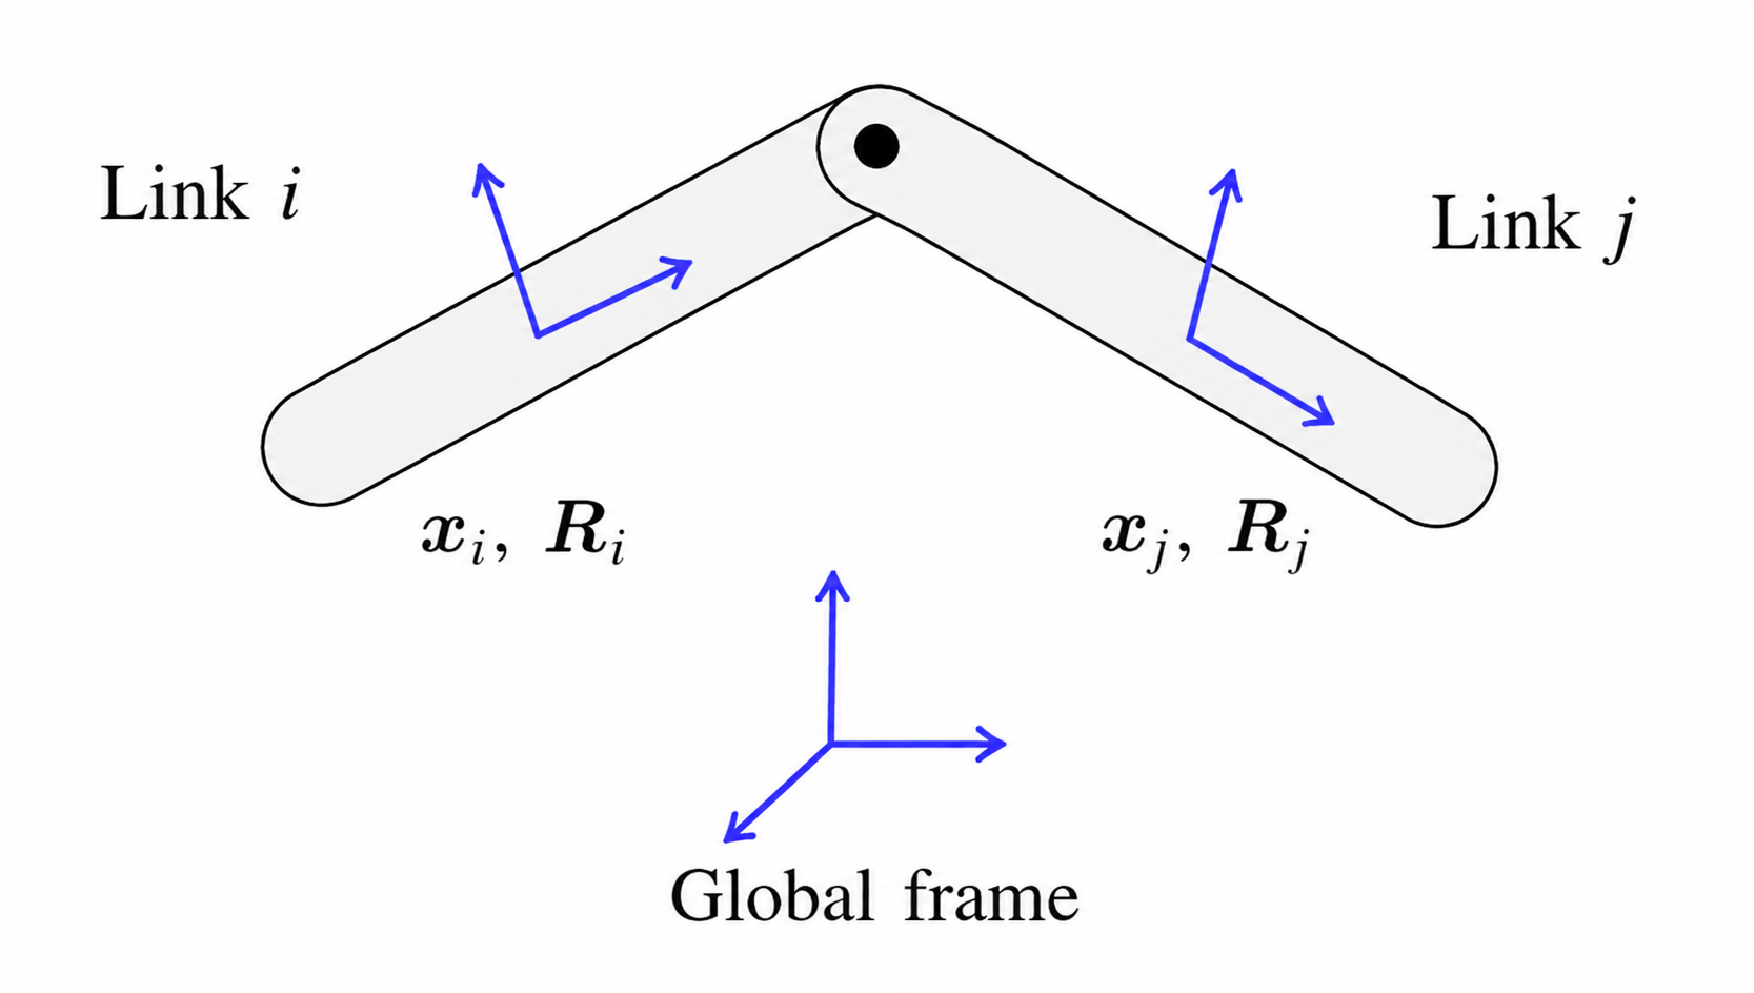
\includegraphics[width=0.60\textwidth]{pics/Maximal_Coordinates_Joint.pdf}
    \caption{Two rigid bodies connected by a holonomic joint in maximal coordinates. Adapted from \cite{BrudigamManchester2021LQR}.}
    \label{fig:maximal_joint_constraint}
\end{figure}

A typical holonomic joint constraint can be written by equating two points
attached to different rigid bodies. This is illustrated in
Fig.~\ref{fig:maximal_joint_constraint}. Let \(\bm{\rho}_i\) and \(\bm{\rho}_j\) denote
constant vectors from the corresponding center of mass to the joint location in
each body-fixed frame. Then a link-connecting constraint is given by
\begin{equation}
    \bm{\phi}_{ij}(q)
    =
    \bm{x}_i+\bm{R}_i\bm{\rho}_i
    -
    \bm{x}_j-\bm{R}_j\bm{\rho}_j
    =
    \bm{0}.
    \label{eq:general_joint_constraint_maximal}
\end{equation}
To include the holonomic constraints in the discrete variational principle, the
discrete action sum is augmented by Lagrange multipliers
\(\bm{\lambda}_k\in\mathbb{R}^{n_c}\). Using a trapezoidal approximation for the
constraint contribution gives
\begin{equation}
    S_{d}
    =
    \sum_{k=0}^{N-1}
    \left[
    L_d(q_k,q_{k+1})
    +
    \frac{h}{2}
    \left(
    \bm{\lambda}_k^\top \bm{\phi}(q_k)
    +
    \bm{\lambda}_{k+1}^\top \bm{\phi}(q_{k+1})
    \right)
    \right].
    \label{eq:constrained_discrete_action}
\end{equation}
The variation with respect to \(q_k\), together with the discrete
Lagrange--d'Alembert force contribution introduced in
Section~\ref{sec:forced_discrete_euler_lagrange}, yields the forced and
constrained discrete Euler-Lagrange equations
\begin{equation}
    D_1 L_d(q_k,q_{k+1})
    +
    D_2 L_d(q_{k-1},q_k)
    +
    \bm{u}_k
    -
    h\,\bm{G}(q_k)^\top \bm{\lambda}_k = 0,
    \qquad
    \bm{\phi}(q_k)=\bm{0},
    \label{eq:forced_constrained_del_general}
\end{equation}
where
\begin{equation}
    \bm{G}(q_k)
    =
    \frac{\partial \bm{\phi}(q_k)}{\partial q_k}
    \label{eq:constraint_jacobian_general}
\end{equation}
denotes the constraint Jacobian.
Equation~\eqref{eq:forced_constrained_del_general} provides the general
forced and constrained discrete Euler-Lagrange equation used for deriving multi-body dynamics.

\subsection{Acrobot}

\paragraph{Configuration Manifold}

\begin{figure}[t]
    \centering
    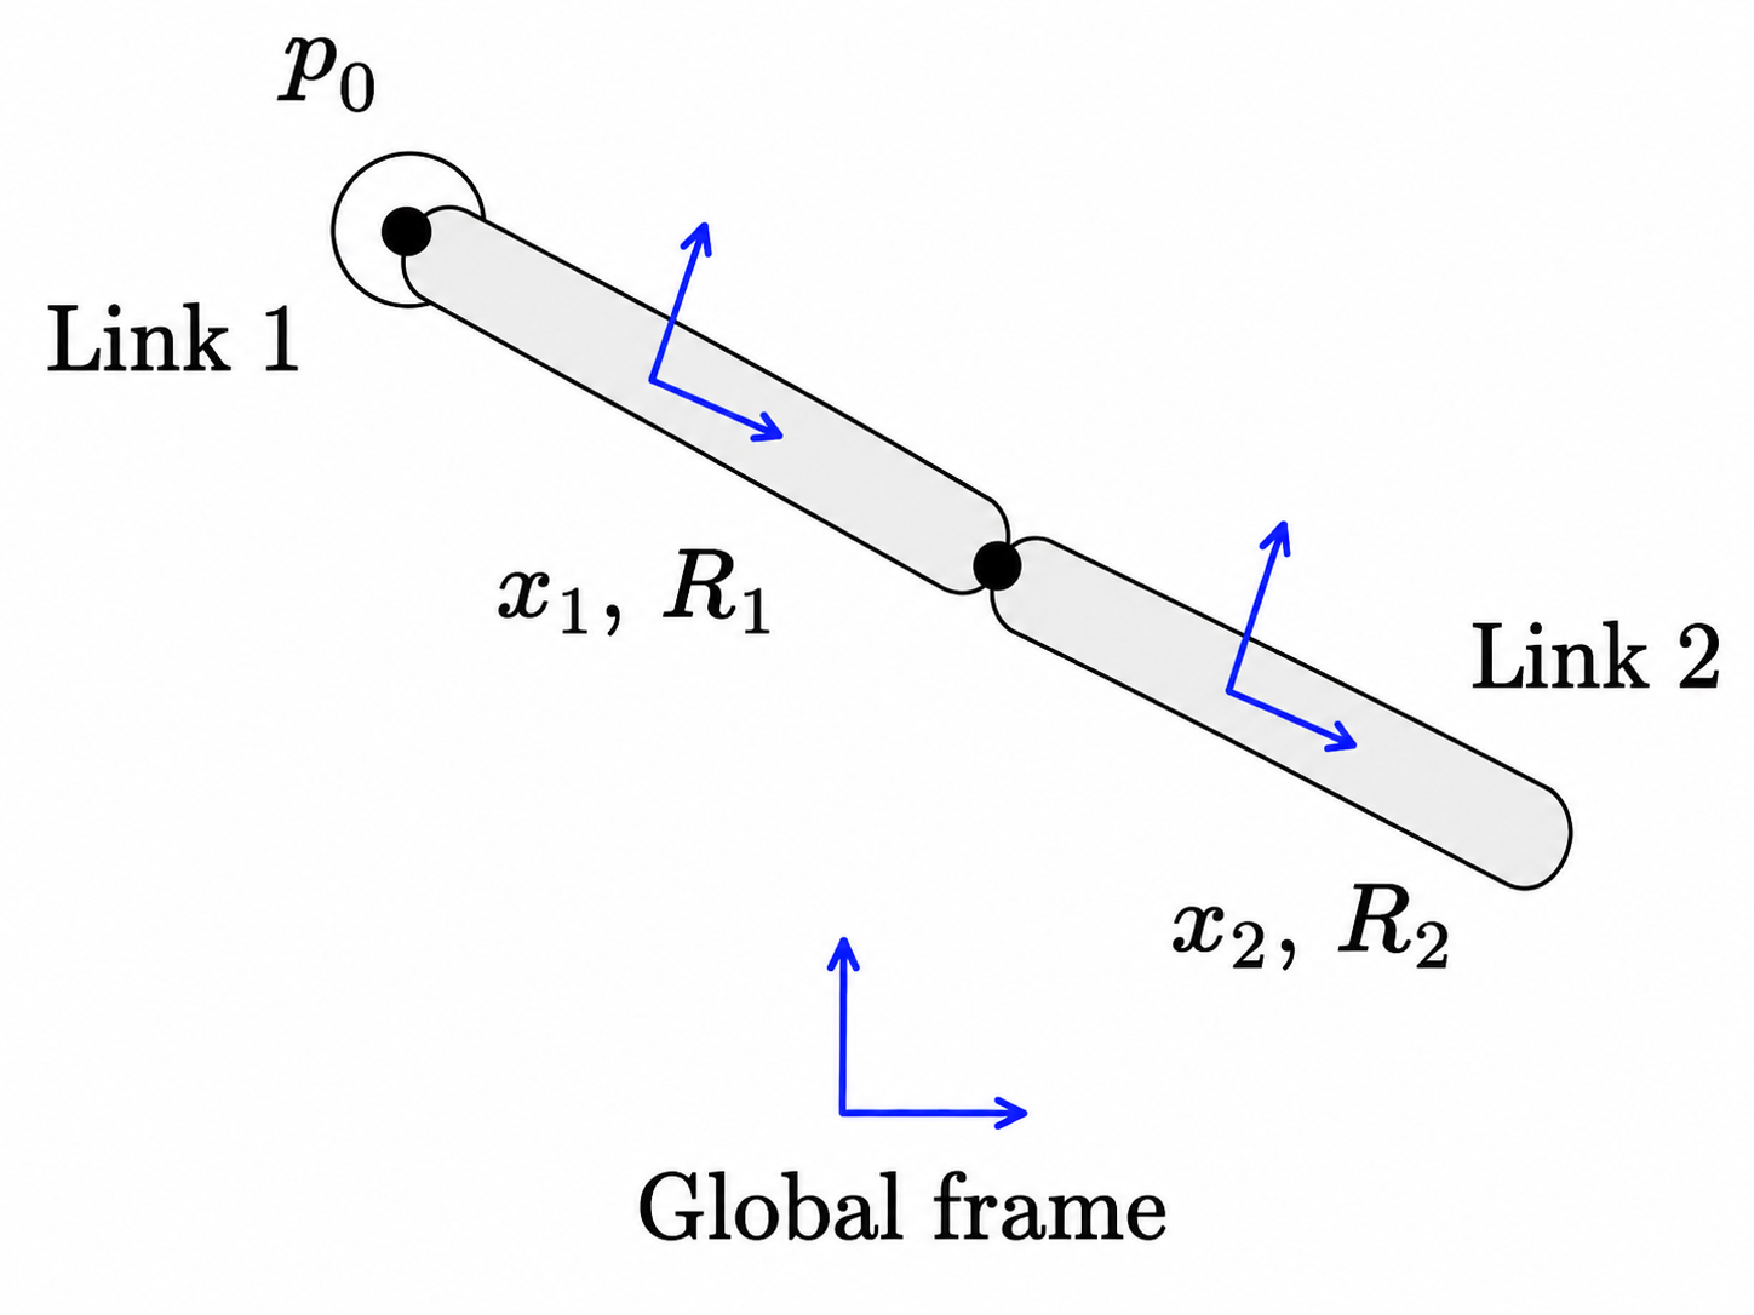
\includegraphics[width=0.50\textwidth]{pics/Acrobot.pdf}
    \caption{Acrobot configuration manifold in maximal coordinates.}
    \label{fig:acrobot_maximal_coordinates}
\end{figure}

The Acrobot model, illustrated in Fig.~\ref{fig:acrobot_maximal_coordinates},
consists of two planar rigid links connected by a revolute joint. The first link is
attached to the inertial frame by a fixed revolute joint, while the second link is
connected to the first link at the elbow. In contrast to the 3D-pendulum, the
system is described in maximal coordinates. Therefore, each link is assigned its own
center of mass position and orientation.

For each link \(i\in\{1,2\}\), the center of mass position is denoted by
\(\bm{x}_i\in\mathbb{R}^2\), and the orientation of the body-fixed frame with
respect to the inertial frame is described by the rotation matrix
\(\bm{R}_i\in SO(2)\). The special orthogonal group in two dimensions is defined as
\begin{equation}
    SO(2)
    =
    \left\{
    \bm{R}\in\mathbb{R}^{2\times 2}
    \mid
    \bm{R}^{\top}\bm{R}=\bm{I}_{2},
    \ \det(\bm{R})=1
    \right\}.
    \label{eq:so2_definition}
\end{equation}
Every element \(\bm{R}_i\in SO(2)\) can be written in terms of an angle
\(\theta_i\in\mathbb{R}\) as
\begin{equation}
    \bm{R}_i
    =
    \begin{bmatrix}
        \cos\theta_i & -\sin\theta_i \\
        \sin\theta_i &  \cos\theta_i
    \end{bmatrix}.
    \label{eq:so2_rotation_matrix}
\end{equation} 
Thus, the unconstrained maximal-coordinate configuration
manifold is given by
\begin{equation}
    Q_{\mathrm{max}}
    =
    \left(
    \mathbb{R}^2 \times SO(2)
    \right)^2 .
    \label{eq:acrobot_q_max}
\end{equation}
The configuration of the Acrobot is written as
\begin{equation}
    q
    =
    \left(
    \bm{x}_1,\bm{R}_1,\bm{x}_2,\bm{R}_2
    \right)
    \in Q_{\mathrm{max}} .
    \label{eq:acrobot_configuration}
\end{equation}
Here, \(\bm{R}_i\) maps vectors from the \(i\)-th body-fixed frame to the inertial
frame.

Let \(\bm{\rho}_{1,0}\in\mathbb{R}^2\) denote the vector from the center of mass of
link~1 to the base joint, expressed in the first body-fixed frame. Furthermore, let
\(\bm{\rho}_{1,12}\in\mathbb{R}^2\) and \(\bm{\rho}_{2,12}\in\mathbb{R}^2\) denote the
vectors from the corresponding centers of mass to the elbow joint, expressed in
the body-fixed frames of link~1 and link~2. The fixed base joint is imposed by
\begin{equation}
    \bm{\phi}_{0}(q)
    =
    \bm{x}_1
    +
    \bm{R}_1\bm{\rho}_{1,0}
    -
    \bm{p}_0
    =
    \bm{0},
    \label{eq:acrobot_base_constraint}
\end{equation}
where \(\bm{p}_0\in\mathbb{R}^2\) is the fixed base position in the inertial frame.
The elbow joint is imposed by requiring the two joint points on link~1 and link~2
to coincide, yielding
\begin{equation}
    \bm{\phi}_{12}(q)
    =
    \bm{x}_1
    +
    \bm{R}_1\bm{\rho}_{1,12}
    -
    \bm{x}_2
    -
    \bm{R}_2\bm{\rho}_{2,12}
    =
    \bm{0}.
    \label{eq:acrobot_elbow_constraint}
\end{equation}
Consequently, the full holonomic constraint vector is defined as
\begin{equation}
    \bm{\phi}(q)
    =
    \begin{bmatrix}
        \bm{\phi}_{0}(q) \\
        \bm{\phi}_{12}(q)
    \end{bmatrix}
    =
    \bm{0}.
    \label{eq:acrobot_constraints}
\end{equation}

In the discrete setting, the attitude of each link is updated by a relative rotation
\(\bm{F}_{i,k}\in SO(2)\), such that
\begin{equation}
    \bm{R}_{i,k+1}
    =
    \bm{R}_{i,k}\bm{F}_{i,k},
    \qquad i\in\{1,2\}.
    \label{eq:acrobot_rotation_update}
\end{equation}
The discrete configuration at time step \(k\) is therefore
\begin{equation}
    q_k
    =
    \left(
    \bm{x}_{1,k},\bm{R}_{1,k},
    \bm{x}_{2,k},\bm{R}_{2,k}
    \right)
    \in Q_c .
    \label{eq:acrobot_discrete_configuration}
\end{equation}

\paragraph{Continuous Lagrangian}

To derive the continuous Lagrangian of the Acrobot in maximal coordinates, the
kinetic and potential energy of both rigid links are introduced. For each link
\(i\in\{1,2\}\), the translational velocity of the center of mass is denoted by
\(\dot{\bm{x}}_i=\bm{v}_i\in\mathbb{R}^2\). Let $\bm{M}_i = m_i\bm{I}_2$ be the mass matrix of link \(i\), and let \(\bm{J}_{d,i}\in\mathbb{R}^{2\times 2}\)
denote the non-standard inertia matrix, similar to Section \ref{sec:discrete_3D_pendulum}. Then, the
kinetic energy with its translational $T_T$ and rotational $T_R$ components is written as
\begin{equation}
    T
    =
    \underbrace{
    \sum_{i=1}^{2}
    \frac{1}{2}\bm{v}_i^{\top}\bm{M}_i\bm{v}_i
    }_{T_T}
    +
    \underbrace{
    \sum_{i=1}^{2}
    \frac{1}{2}
    \mathrm{tr}
    \left[
        \hat{\omega}_i
        \bm{J}_{d,i}
        \hat{\omega}_i^{\top}
    \right]
    }_{T_R}.
    \label{eq:acrobot_kinetic_energy_split}
\end{equation}
The gravitational potential energy is expressed directly by the center of mass
positions. In contrast to the 3D-pendulum, zero potential is assumed for the rotational setting \cite{BrudigamManchester2021VariationalIntegrators}, 
which gives 
\begin{equation}
    V_R(\bm{R}_1,\bm{R}_2)=0.
    \label{eq:acrobot_rotation_potential_zero}
\end{equation}
Therefore, the gravitational potential energy is given by the translational case
\begin{equation}
    V_T(\bm{x}_1,\bm{x}_2)
    =
    \sum_{i=1}^{2}
    g\,\bm{e}_2^{\top}\bm{M}_i\bm{x}_i,
    \label{eq:acrobot_potential_energy}
\end{equation}
where \(\bm{e}_2\in\mathbb{R}^2\) denotes the vertical unit vector in the inertial frame.
Consequently, the continuous Lagrangian
\(L:TQ_{\mathrm{max}}\rightarrow\mathbb{R}\) is defined as
\begin{equation}
    \begin{aligned}
    L(q,\dot{q})
    &=
    \sum_{i=1}^{2}
    \left(
    \frac{1}{2}\bm{v}_i^{\top}\bm{M}_i\bm{v}_i
    +
    \frac{1}{2}
    \mathrm{tr}
    \left[
        \hat{\omega}_i
        \bm{J}_{d,i}
        \hat{\omega}_i^{\top}
    \right]
    \right)
    -
    \sum_{i=1}^{2}
    g\,\bm{e}_2^{\top}\bm{M}_i\bm{x}_i .
    \end{aligned}
    \label{eq:acrobot_continuous_lagrangian}
\end{equation}

\paragraph{Discrete Lagrangian}

For the Acrobot in maximal coordinates, the translational and rotational parts are
discretized separately, following the structure of maximal-coordinate variational
integrators in \cite{BrudigamManchester2021VariationalIntegrators}. Therefore,
the discrete Lagrangian is written as
\begin{equation}
    L_d(q_k,q_{k+1})
    =
    T_{d,T}(q_k,q_{k+1})
    +
    T_{d,R}(q_k,q_{k+1})
    -
    V_{d,T}(q_k,q_{k+1}).
    \label{eq:acrobot_discrete_lagrangian_split}
\end{equation}

For the translational part, the center of mass velocity of each link is approximated
by
\begin{equation}
    \bm{v}_{i,k}
    \approx
    \frac{\bm{x}_{i,k+1}-\bm{x}_{i,k}}{h},
    \qquad i\in\{1,2\}.
    \label{eq:acrobot_discrete_translational_velocity}
\end{equation}
\cite{BrudigamManchester2021VariationalIntegrators} defines the discrete translational kinetic energy contribution to be
\begin{equation}
    T_{d,T}(q_k,q_{k+1})
    =
    \sum_{i=1}^{2}
    \frac{1}{2h}
    \left(
    \bm{x}_{i,k+1}-\bm{x}_{i,k}
    \right)^{\top}
    \bm{M}_i
    \left(
    \bm{x}_{i,k+1}-\bm{x}_{i,k}
    \right).
    \label{eq:acrobot_discrete_translational_lagrangian}
\end{equation}
Substituting the angular velocity approximation \eqref{eq:discrete_velocity_approximation} into the rotational kinetic energy
$T_R$ of \eqref{eq:acrobot_kinetic_energy_split}, the discrete rotational kinetic
energy contribution is derived to
\begin{equation}
\begin{aligned}
    T_{d,R}(q_k,q_{k+1})
    &=
    \sum_{i=1}^{2}
    \frac{1}{2h}
    \mathrm{tr}
    \left[
    \left(
    \bm{F}_{i,k}-\bm{I}_{2}
    \right)
    \bm{J}_{d,i}
    \left(
    \bm{F}_{i,k}-\bm{I}_{2}
    \right)^{\top}
    \right] \\
    &=
    \sum_{i=1}^{2}
    \frac{1}{h}
    \mathrm{tr}
    \left[
    \left(
    \bm{I}_{2}
    -
    \bm{F}_{i,k}
    \right)
    \bm{J}_{d,i}
    \right].
\end{aligned}
\label{eq:acrobot_discrete_rotational_lagrangian}
\end{equation}
which calculation corresponds to the discrete rotational kinetic energy of the 3D-pendulum in Section \ref{sec:discrete_3D_pendulum}.

Finally, using the trapezoidal rule for the discretization of the potential energy integral, the discrete translational potential contribution $V_{d,T}$
is given by
\begin{equation}
    V_{d,T}(q_k,q_{k+1})
    =
    \frac{h}{2}
    \sum_{i=1}^{2}
    m_i g
    \bm{e}_{2}^{\top}
    \left(
    \bm{x}_{i,k}
    +
    \bm{x}_{i,k+1}
    \right).
    \label{eq:acrobot_discrete_potential_lagrangian}
\end{equation}

Combining the translational \eqref{eq:acrobot_discrete_translational_lagrangian}, rotational \eqref{eq:acrobot_discrete_rotational_lagrangian}, and potential \eqref{eq:acrobot_discrete_potential_lagrangian} contributions gives the
discrete Lagrangian
\begin{equation}
    \begin{aligned}
    L_d(q_k,q_{k+1})
    =
    &
    \text{  }
    L_d
    \left(
    \bm{x}_{1,k},\bm{x}_{1,k+1},
    \bm{x}_{2,k},\bm{x}_{2,k+1},
    \bm{F}_{1,k},\bm{F}_{2,k}
    \right)  \\
    =
    &
    \sum_{i=1}^{2}
    \frac{1}{2h}
    \left(
    \bm{x}_{i,k+1}-\bm{x}_{i,k}
    \right)^{\top}
    \bm{M}_i
    \left(
    \bm{x}_{i,k+1}-\bm{x}_{i,k}
    \right)  \\
    &
    +
    \sum_{i=1}^{2}
    \frac{1}{h}
    \mathrm{tr}
    \left[
    \left(
    \bm{I}_{2}
    -
    \bm{F}_{i,k}
    \right)
    \bm{J}_{d,i}
    \right]   \\
    &
    -
    \frac{h}{2}
    \sum_{i=1}^{2}
    g
    \bm{e}_{2}^{\top}
    \bm{M}_i
    \left(
    \bm{x}_{i,k}
    +
    \bm{x}_{i,k+1}
    \right).
    \end{aligned}
    \label{eq:acrobot_discrete_lagrangian}
\end{equation}

\paragraph{Discrete Euler-Lagrange Equations}

The discrete equations of motion are obtained from the stationary condition of the
constrained discrete action. 
The holonomic constraints introduced in
\eqref{eq:acrobot_constraints} are included by extending the action integral with
Lagrange multipliers. Let
\begin{equation}
    \bm{\lambda}
    =
    \begin{bmatrix}
        \bm{\lambda}_{0} \\
        \bm{\lambda}_{12}
    \end{bmatrix}
    \in\mathbb{R}^{4},
    \label{eq:acrobot_lagrange_multipliers}
\end{equation}
where \(\bm{\lambda}_{0}\in\mathbb{R}^2\) enforces the base constraint and
\(\bm{\lambda}_{12}\in\mathbb{R}^2\) enforces the elbow constraint.
Using the constrained action sum defined in \eqref{eq:constrained_discrete_action}, the
variation is written as
\begin{equation}
    \delta S_{d}
    =
    \delta
    \sum_{k=0}^{N-1}
    \left[
    L_d(q_k,q_{k+1})
    +
    \frac{h}{2}
    \left(
    \bm{\lambda}_{k}^{\top}\bm{\phi}(q_k)
    +
    \bm{\lambda}_{k+1}^{\top}\bm{\phi}(q_{k+1})
    \right)
    \right]
    = 0.
    \label{eq:acrobot_variation_constrained_discrete_action}
\end{equation}
The translational and rotational components are treated separately, following the
maximal-coordinate variational-integrator structure. In \cite{BrudigamManchester2021VariationalIntegrators},
the variation of the translational component is given as
\begin{equation}
    \delta_{\bm{x}_{i,k+1}} S_{d,c}
    =
    \left\langle
    \frac{1}{h}\bm{M}_i
    \left(
    \bm{v}_{i,k}
    -
    \bm{v}_{i,k+1}
    \right)
    -
    g\bm{M}_i\bm{e}_2
    +
    \bm{G}_{x_i,k+1}^{\top}\bm{\lambda}_{k+1},
    \delta\bm{x}_{i,k+1}
    \right\rangle .
    \label{eq:acrobot_translational_variation}
\end{equation}
using the relation \eqref{eq:acrobot_discrete_translational_velocity}.
The constraint contribution is calculated to
\begin{equation}
    \bm{G}_{x,k+1}^{\top}\bm{\lambda}_{k+1}
    =
    \begin{bmatrix}
        \dfrac{\partial \bm{\phi}_{0,k+1}}{\partial \bm{x}_{1,k+1}}
        &
        \dfrac{\partial \bm{\phi}_{0,k+1}}{\partial \bm{x}_{2,k+1}}
        \\[0.8em]
        \dfrac{\partial \bm{\phi}_{12,k+1}}{\partial \bm{x}_{1,k+1}}
        &
        \dfrac{\partial \bm{\phi}_{12,k+1}}{\partial \bm{x}_{2,k+1}}
    \end{bmatrix}^{\top}
    \begin{bmatrix}
        \bm{\lambda}_{0,k+1} \\
        \bm{\lambda}_{12,k+1}
    \end{bmatrix}  
    =
    \begin{bmatrix}
        \bm{\lambda}_{0,k+1}+\bm{\lambda}_{12,k+1} \\
        -\bm{\lambda}_{12,k+1}
    \end{bmatrix}.
    \label{eq:acrobot_translational_constraint_force}
\end{equation}
with the discretized constraints
\begin{equation}
    \bm{\phi}(q_{k+1})
    =
    \begin{bmatrix}
        \bm{\phi}_{0,k+1} \\
        \bm{\phi}_{12,k+1}
    \end{bmatrix}
    =
    \begin{bmatrix}
    \bm{x}_{1,k+1}
    +
    \bm{R}_{1,k+1}\bm{\rho}_{1,0}
    -
    \bm{p}_0
    \\
    \bm{x}_{1,k+1}
    +
    \bm{R}_{1,k+1}\bm{\rho}_{1,12}
    -
    \bm{x}_{2,k+1}
    -
    \bm{R}_{2,k+1}\bm{\rho}_{2,12}
    \end{bmatrix}.
    \label{eq:acrobot_discrete_constraints_vector}
\end{equation}
Therefore, substituting the gradient \eqref{eq:acrobot_translational_constraint_force} into \eqref{eq:acrobot_translational_variation}, the translational discrete Euler-Lagrange equations for link 1 and link 2 are
\begin{subequations}
\label{eq:acrobot_translational_del_links}
\begin{align}
    \frac{1}{h}\bm{M}_{1}
    \left(
    \bm{v}_{1,k+1}
    -
    \bm{v}_{1,k}
    \right)
    +
    g\bm{M}_{1}\bm{e}_{2}
    -
    \left(
    \bm{\lambda}_{0,k+1}
    +
    \bm{\lambda}_{12,k+1}
    \right)
    &=
    \bm{0},
    \label{eq:acrobot_translational_del_link_1}
    \\
    \frac{1}{h}\bm{M}_{2}
    \left(
    \bm{v}_{2,k+1}
    -
    \bm{v}_{2,k}
    \right)
    +
    g\bm{M}_{2}\bm{e}_{2}
    +
    \bm{\lambda}_{12,k+1}
    &=
    \bm{0}.
    \label{eq:acrobot_translational_del_link_2}
\end{align}
\end{subequations}

For the rotational part, the derivatives of \ref{eq:euler} have to be taken for each link, analogously to the 3D-pendulum of Section \ref{sec:discrete_3D_pendulum}.
Firstly, the directional derivative $\left\langle D_{\bm{F_{i,k}}}L_d(\bm{F}_{i,k}), \delta \bm{f}_{i,k} \right\rangle$ is given by applying \eqref{eq:derivative_fk}, which yields to
\begin{equation}
    \begin{aligned}
    \left\langle
    T_e^*L_{\bm{F}_{i,k}}
    D_{\bm{F}_{i,k}}L_{d,R,i},
    \hat{\chi}_k
    \right\rangle
    &=
    \left.
    \frac{d}{d\epsilon}
    \right|_{\epsilon=0}
    L_{d}
    \left(
    \bm{F}_{i,k}
    \exp(\epsilon\hat{\chi}_k)
    \right)
    \\
    &=
    -
    \frac{1}{h}
    \mathrm{tr}
    \left[
    \bm{F}_{i,k}
    \hat{\chi}_k
    \bm{J}_{d,i}
    \right]
    \\
    &=
    \left\langle
    \frac{1}{h}
    \left(
    \bm{J}_{d,i}\bm{F}_{i,k}
    -
    \bm{F}_{i,k}^{\top}\bm{J}_{d,i}
    \right),
    \hat{\chi}_k
    \right\rangle
    \\
    &=
    \left\langle
    \bm{\Pi}_{i,k}
    ,
    \hat{\chi}_k
    \right\rangle
    , 
    \end{aligned}
    \label{eq:acrobot_rotational_derivative_pairing}
\end{equation}
corresponding to the derivative of the single body 3D-pendulum derived in Section \ref{sec:discrete_3D_pendulum}. 
Here,
\begin{equation}
    \bm{\Pi}_{i,k}
    =
    \frac{1}{h}
    \left(
        \bm{J}_{d,i}\bm{F}_{i,k}
        -
        \bm{F}_{i,k}^{\top}\bm{J}_{d,i}
    \right),
    \qquad i\in\{1,2\},
    \label{eq:acrobot_discrete_angular_momentum}
\end{equation}
denotes the discrete angular momentum
of link \(i\) associated with the relative rotation\(\bm{F}_{i,k}\).
It is the analogue of the discrete Legendre momentum \eqref{eq:discrete_3D_pendulum_momentum_1} used for
the 3D-pendulum in Section \ref{sec:discrete_3D_pendulum}, now defined separately for each rigid link \cite{Lee2008}.

Since \(SO(2)\) is abelian, it follows that \(\mathrm{Ad}_{\bm{F}_{i,k}}=I\) \cite{Lee2008}.
Therefore, the coadjoint term is equal to \eqref{eq:acrobot_rotational_derivative_pairing} at time step $k+1$, which gives
\begin{equation}\label{eq:acrobot_Ad_variation}
\operatorname{Ad}^{*}_{\bm{F}_{i,k+1}^{-1}}
\!\left(
T_e^*L_{\bm{F}_{i,k+1}}
D_{\bm{F}_{i,k+1}}L_d(\bm{F}_{i,k+1})
\right)
= 
\frac{1}{h}
\left(
\bm{J}_{d,i}\bm{F}_{i,k+1}
-
\bm{F}_{i,k+1}^{\top}\bm{J}_{d,i}
\right).
\end{equation}
It remains to derive the directional derivative of the rotations $R_{i,k+1}$. 
From \eqref{eq:acrobot_variation_constrained_discrete_action}, it is observed that only the constraints $\bm{\phi}(q_k)$ are dependent on
the rotation matrices \(\bm{R}_{1,k}\) and \(\bm{R}_{2,k}\). 
Hence, the variation of the constraint contribution 
\begin{equation*}
    \left\langle D_{\bm{R}_{i,k+1}}(h \bm{\lambda}_{k+1}^\top \bm{\phi}_{k+1}), \delta \bm{R}_{i,k+1} \right\rangle=\left\langle T_e^* L_{\bm{R}_{i,k+1}} D_{\bm{R}_{i,k+1}}(h \bm{\lambda}_{k+1}^\top \bm{\phi}_{k+1}), \hat{\eta}_{i,k+1} \right\rangle,
\end{equation*}
has to be evaluated for each link $i$, using \eqref{eq:derivative_gk}. For link $i=1$, the variation of the constraint contribution is given by
\begin{equation}
    \begin{aligned}
    &
    \left\langle
    T_e^*L_{\bm{R}_{1,k+1}}
    D_{\bm{R}_{1,k+1}}
    \left(
    h\bm{\lambda}_{k+1}^{\top}\bm{\phi}_{k+1}
    \right),
    \hat{\eta}_{1,k+1}
    \right\rangle
    \\
    &=
    \left.
    \frac{d}{d\epsilon}
    \right|_{\epsilon=0}
    h
    \left[
    \bm{\lambda}_{0,k+1}^{\top}
    \bm{\phi}_{0,k+1}^{\epsilon}
    +
    \bm{\lambda}_{12,k+1}^{\top}
    \bm{\phi}_{12,k+1}^{\epsilon}
    \right]
    \\
    &=
    h 
    \left[
    \bm{\lambda}_{0,k+1}^{\top}
    \bm{R}_{1,k+1}\hat{\eta}_{1,k+1}\bm{\rho}_{1,0}
    +
    \bm{\lambda}_{12,k+1}^{\top}
    \bm{R}_{1,k+1}\hat{\eta}_{1,k+1}\bm{\rho}_{1,12}
    \right]
    \\
    &=
    h
    \left[
    \left(
    \bm{\rho}_{1,0}
    \times
    \bm{R}_{1,k+1}^{\top}\bm{\lambda}_{0,k+1}
    \right)
    +
    \left(
    \bm{\rho}_{1,12}
    \times
    \bm{R}_{1,k+1}^{\top}\bm{\lambda}_{12,k+1}
    \right)
    \right]
    \cdot
    \eta_{1,k+1}
    \\
    &=
    \left\langle
    h
    \left[
    \left(
    \bm{\rho}_{1,0}
    \times
    \bm{R}_{1,k+1}^{\top}\bm{\lambda}_{0,k+1}
    \right)
    +
    \left(
    \bm{\rho}_{1,12}
    \times
    \bm{R}_{1,k+1}^{\top}\bm{\lambda}_{12,k+1}
    \right)
    \right]^{\wedge},
    \hat{\eta}_{1,k+1}
    \right\rangle,
    \end{aligned}
    \label{eq:acrobot_R1_constraint_derivative_kp1}
\end{equation}
which calculation corresponts to the derivative of the 3D-pendulum with respect to the rotation matrix $R_k$ derived in Section \ref{sec:discrete_3D_pendulum}. 
In contrast, the variation of the constraint contribution for link $i=2$ only depends on $\phi_{12,k+1}$ and is derived to
\begin{equation}
    \begin{aligned}
    &
    \left\langle
    T_e^*L_{\bm{R}_{2,k+1}}
    D_{\bm{R}_{2,k+1}}
    \left(
    h\bm{\lambda}_{k+1}^{\top}\bm{\phi}_{k+1}
    \right),
    \hat{\eta}_{2,k+1}
    \right\rangle
    \\
    &=
    \left.
    \frac{d}{d\epsilon}
    \right|_{\epsilon=0}
    h
    \left[
    \bm{\lambda}_{12,k+1}^{\top}
    \bm{\phi}_{12,k+1}^{\epsilon}
    \right]
    \\
    &=
    \left.
    \frac{d}{d\epsilon}
    \right|_{\epsilon=0}
    h
    \left[
    \bm{\lambda}_{12,k+1}^{\top}
    \left(
    -
    \bm{R}_{2,k+1}
    \exp(\epsilon\hat{\eta}_{2,k+1})
    \bm{\rho}_{2,12}
    \right)
    \right]
    \\
    &=
    -h
    \left[
    \bm{\lambda}_{12,k+1}^{\top}
    \bm{R}_{2,k+1}
    \hat{\eta}_{2,k+1}
    \bm{\rho}_{2,12}
    \right]
    \\
    &=
    -h
    \left(
    \bm{\rho}_{2,12}
    \times
    \bm{R}_{2,k+1}^{\top}\bm{\lambda}_{12,k+1}
    \right)
    \cdot
    \eta_{2,k+1}
    \\
    &=
    \left\langle
    -h
    \left(
    \bm{\rho}_{2,12}
    \times
    \bm{R}_{2,k+1}^{\top}\bm{\lambda}_{12,k+1}
    \right)^{\wedge},
    \hat{\eta}_{2,k+1}
    \right\rangle .
    \end{aligned}
    \label{eq:acrobot_R2_constraint_derivative_kp1}
\end{equation}

The full rotational contribution is described, by substituting \eqref{eq:acrobot_rotational_derivative_pairing}, \eqref{eq:acrobot_Ad_variation}, \eqref{eq:acrobot_R1_constraint_derivative_kp1} and \eqref{eq:acrobot_R2_constraint_derivative_kp1} for each link $i = 1,2$ into \eqref{eq:discrete_euler_lagrange}. Moreover, \eqref{eq:acrobot_translational_derivative} gives the translational description.
Finally, the full discrete Euler-Lagrange equations of the unforced Acrobot in maximal coordinates are expressed on \(\left(\mathbb{R}^2\times SO(2)\right)^2\) as
\begin{subequations}
\label{eq:acrobot_full_del_shifted}
\begingroup
\small
\setlength{\jot}{0.35em}
\vspace{-0.3cm}
\begin{align}
    \intertext{\textit{Translation:}}
    \vspace{-0.1cm}
    \frac{1}{h}\bm{M}_{1}
    \left(
        \bm{v}_{1,k+1}
        -
        \bm{v}_{1,k}
    \right)
    +
    g\bm{M}_{1}\bm{e}_2
    -
    \left(
        \bm{\lambda}_{0,k+1}
        +
        \bm{\lambda}_{12,k+1}
    \right)
    &=
    \bm{0},
    \label{eq:acrobot_full_del_shifted_translation_1}
    \\
\hspace{-2em}
    \frac{1}{h}\bm{M}_{2}
    \left(
        \bm{v}_{2,k+1}
        -
        \bm{v}_{2,k}
    \right)
    +
    g\bm{M}_{2}\bm{e}_2
    +
    \bm{\lambda}_{12,k+1}
    &=
    \bm{0},
    \label{eq:acrobot_full_del_shifted_translation_2}
\end{align}
\vspace{-0.4cm}
\vspace{-0.6cm}
\begin{align}
    \intertext{\textit{Rotation:}}
    \vspace{-0.1cm}
    \bm{\Pi}_{1,k}
    -
    \bm{\Pi}_{1,k+1}
    +
    h
    \left[
    \left(
    \bm{\rho}_{1,0}
    \times
    \bm{R}_{1,k+1}^{\top}\bm{\lambda}_{0,k+1}
    \right)
    +
    \left(
    \bm{\rho}_{1,12}
    \times
    \bm{R}_{1,k+1}^{\top}\bm{\lambda}_{12,k+1}
    \right)
    \right]^{\wedge}
    &=
    \bm{0},
    \label{eq:acrobot_full_del_shifted_rotation_1}
    \\
\hspace{-2em}
    \bm{\Pi}_{2,k}
    -
    \bm{\Pi}_{2,k+1}
    -
    h
    \left[
    \left(
    \bm{\rho}_{2,12}
    \times
    \bm{R}_{2,k+1}^{\top}\bm{\lambda}_{12,k+1}
    \right)
    \right]^{\wedge}
    &=
    \bm{0},
    \label{eq:acrobot_full_del_shifted_rotation_2}
\end{align}
\vspace{-0.4cm}
\vspace{-0.6cm}
\begin{align}
    \intertext{\textit{Constraints:}}    
    \bm{\phi}_{0,k+1}
    =
    \bm{x}_{1,k+1}
    +
    \bm{R}_{1,k+1}\bm{\rho}_{1,0}
    -
    \bm{p}_0
    &=
    \bm{0},
    \label{eq:acrobot_full_del_shifted_base_constraint}
    \\
\hspace{-2em}
    \bm{\phi}_{12,k+1}
    =
    \bm{x}_{1,k+1}
    +
    \bm{R}_{1,k+1}\bm{\rho}_{1,12}
    -
    \bm{x}_{2,k+1}
    -
    \bm{R}_{2,k+1}\bm{\rho}_{2,12}
    &=
    \bm{0},
    \label{eq:acrobot_full_del_shifted_elbow_constraint}
\end{align}
\vspace{-0.4cm}    
\vspace{-0.6cm}
\begin{align}
    \intertext{\textit{Kinematics:}}    
    \bm{R}_{1,k+1}
    &=
    \bm{R}_{1,k}\bm{F}_{1,k},
    \label{eq:acrobot_full_del_shifted_kinematics_1}
    \\
\hspace{-2em}
    \bm{R}_{2,k+1}
    &=
    \bm{R}_{2,k}\bm{F}_{2,k}.
    \label{eq:acrobot_full_del_shifted_kinematics_2}
\end{align}
\endgroup
\end{subequations}
in dependence to its constraints \eqref{eq:acrobot_constraints}.

\paragraph{Controlled Acrobot}

As in the controlled 3D-pendulum case (Section \ref{sec:discrete_3D_pendulum}), the trapezoidal approximation distributes
the virtual work equally to both endpoints of the interval. Therefore, the discrete
Legendre force contributions of \eqref{eq:discrete_forces_special} are given by
\begin{equation}
    u_{d,k}^{-}=u_{d,k}^{+}=\frac{h}{2}u_k .
\end{equation}
The Acrobot is actuated by a single motor located at the elbow joint \cite{BrudigamManchester2021LQR}. In contrast
to the controlled 3D-pendulum, the input is therefore not an external moment acting
on one rigid body, but an internal joint torque acting between the two links. The generalized torque vector
is defined as
\begin{equation}
    \bm{\tau}_k
    =
    \begin{bmatrix}
        -u_k \\
         u_k
    \end{bmatrix},
    \label{eq:acrobot_generalized_torque}
\end{equation}
with \(u_k\in\mathbb{R}\) being the scalar elbow torque, applying 
opposite moments between the two links.

Since the Acrobot is actuated by a motor at the elbow joint, the control input is a
pure rotational torque acting between the two links. Hence, there is no external
translational force acting directly on the centers of mass, and the translational
force contribution is set to
\begin{equation}
    \bm{f}^{x}_{1,k}
    =
    \bm{f}^{x}_{2,k}
    =
    \bm{0}.
    \label{eq:acrobot_zero_translational_force}
\end{equation}
Using the discrete Lagrange-d'Alembert principle \eqref{eq:forced_discrete_EL_compact}, the generalized torque
contribution \eqref{eq:acrobot_generalized_torque} is added only to the unforced 
rotational equations \eqref{eq:acrobot_full_del_shifted_rotation_1} and \eqref{eq:acrobot_full_del_shifted_rotation_2}. 
Therefore, the controlled rotational discrete Euler-Lagrange equations are derived to
\begin{subequations}
\label{eq:forced_acrobot_rotational_equations}
\begingroup
\footnotesize
\setlength{\jot}{0.25em}
\begin{align}
    \bm{\Pi}_{1,k}
    -
    \bm{\Pi}_{1,k+1}
    +
    h
    \left[
    \left(
    \bm{\rho}_{1,0}
    \times
    \bm{R}_{1,k+1}^{\top}\bm{\lambda}_{0,k+1}
    \right)
    +
    \left(
    \bm{\rho}_{1,12}
    \times
    \bm{R}_{1,k+1}^{\top}\bm{\lambda}_{12,k+1}
    \right)
    -
    u_{k+1}
    \right]^{\wedge}
    &=
    \bm{0},
    \label{eq:forced_acrobot_rotation_link1}
    \\
    \bm{\Pi}_{2,k}
    -
    \bm{\Pi}_{2,k+1}
    +
    h
    \left[
    u_{k+1}
    -
    \left(
    \bm{\rho}_{2,12}
    \times
    \bm{R}_{2,k+1}^{\top}\bm{\lambda}_{12,k+1}
    \right)
    \right]^{\wedge}
    &=
    \bm{0}.
    \label{eq:forced_acrobot_rotation_link2}
\end{align}
\endgroup
\end{subequations}
For \(u_{k+1}=0\), these equations reduce to the corresponding unforced rotational
equations derived previously.

